\section{Analysis Procedure} \label{sec:ana}
The goal of TASEH is to find the axion signal hidden in the noise. In 
order to achieve this, the analysis procedure includes the following steps:
    \begin{enumerate}
        \item Perform fast Fourier transform (FFT) on the 
IQ time series data to obtain the frequency-domain power spectrum.
        \item Apply the Savitzky-Golay (SG) filter to remove the structure 
of the background in the frequency-domain power spectrum.
        \item Combine all the spectra from different frequency scans with 
the weighting algorithm.
        \item Merge bins in the combined spectrum to maximize the SNR. 
       \item Rescan the frequency regions with candidates and set limits on 
      the axion-two-photon coupling \gagg\ if no candidates were found.
    \end{enumerate}

    The analysis follows the procedure similar to that 
developed by the HAYSTAC experiment~\cite{HAYSTACII}. The important points  
and formulas for each step are highlighted below as a reminder 
for the convenience of readers. Note there are a few  
small differences between the HAYSTAC analysis and the one presented here. 
In this paper, the uncertainties are considered to be uncorrelated between 
different frequency bins while Ref.~\cite{HAYSTACII} takes into account 
the correlation. The frequency-domain spectra processed by each intermediate 
step are shown. The central results of the \gagg\ limits assume the signal 
line shape described by Eq.~\eqref{eq:simplesignal} as in 
Ref.~\cite{HAYSTACII}. In addition, the limits without an assumption of 
signal line shape and the limits assuming a 
Gaussian signal with a narrower FWHM are 
shown for comparison in Sec.~\ref{sec:results}. 
As a sanity check, the data are analyzed by two 
independent groups and their results are consistent with each other. 


\subsection{Fast Fourier transform}
\label{sec:FFT}
The in-phase $I(t)$ and quadrature $Q(t)$ components of the time-domain 
data were sampled and saved in the TDMS 
(Technical Data Management Streaming) files - a 
binary format developed by National Instruments. 
The FFT is performed to convert the data into 
frequency-domain power spectrum in which the power is calculated 
using the following equation:

\begin{equation}
\label{eq:4.1}
    \text{Power} = \frac{|\text{FFT}(I+i \cdot Q)|^{2}}{N \cdot 2R},
\end{equation}
where $N$ is the number of data points ($N  = 2000$ in the TASEH 
CD102 data), and $R$ is the input resistance of the signal analyzer 
(50~$\Omega$).
The FFT is done for every one-millisecond subspectrum data. The integration 
time for each frequency scan was about 32-42 minutes, which resulted 
in 1920000 to 2520000 subspectra; an average over these subspectra gives 
the averaged frequency-domain power spectrum for each scan. 
The frequency span in the spectrum from each resonant-frequency scan is 
2~MHz while the resolution is 1~kHz. In order to avoid the aliasing 
effect, a band-pass filter was applied in the data acquisition, 
giving a frequency span of 1.6~MHz (1600 frequency bins) that can be used 
for the analysis. 


\subsection{Remove the structure of the background} 
In the absence of the axion signal, the output data spectrum is simply the 
noise from the cavity and the amplification chain. If axions are present 
in the cavity, the signal will be buried in the noise because the 
signal power is very weak. Therefore, the structure of the raw averaged 
output power spectrum, as shown in the upper left panel of 
Fig.~\ref{fig:raw_sg_power}, is dominated 
by the noise of the system and an explanation for the structure can be found 
in Appendix~\ref{sec:cavitynoise}. The SG 
filter~\cite{SGFilter}, a digital filter that can smooth data without 
distorting the signal tendency, is applied to remove the structure of the  
background. The SG filter is performed on the averaged spectrum of each 
frequency scan by fitting adjacent points of successive sub-sets of data with 
an $n^\text{th}$-order polynomial. The result depends on two parameters: 
the number of 
data points used for fitting, the so-called window width, and the order of 
the polynomial. If the window is too wide, the filter will not remove small 
structures, and if it is too narrow, it may kill the signal. 
A window width of 201 frequency bins and a 4$^\text{th}$-order polynomial 
were first chosen during the data taking, by 
requiring the ratio of the raw data to the filter 
output consistent with unity.  
The SG-filter parameters 
are also cross-checked using 10000 pseudo-experiments that include simulations 
of the noise spectrum and an axion signal with 
$\ggamma\approx 10 \left|g_\text{KSVZ}\right|$; the measured signal power 
is found to be consistent with the injected one within 1\%.


The SG-filter output can be considered as the averaged noise power. 
The raw averaged power spectrum is divided by the output of the SG filter, 
then unity is subtracted from the ratio to get the dimensionless 
normalized spectrum (lower left panel of Fig.~\ref{fig:raw_sg_power}). 
The relative deviation of power (RDP) in the normalized spectrum (and also in 
the spectra processed with rescaling, combining, and merging afterwards) are 
denoted by the symbol $\delta$. The values of 
RDPs can be zero, positive, or negative. 
In the absence of the axion signal, the RDPs in the normalized spectrum are 
samples drawn from a Gaussian 
distribution with a zero mean and a standard deviation of 
$\left.1\middle/\sqrt{N_\text{spectra}}\right.$, where $N_\text{spectra}$ is 
the number of subspectra used to compute the average (see Sec.~\ref{sec:FFT} 
and the right panel of Fig.~\ref{fig:raw_sg_power}). 

The normalized spectrum from each scan is further rescaled 
 with the following formula:
\begin{equation}
  \label{eq:respower_eqn}
  \delta_{ij}^\text{res} = R_{ij}\delta_{ij}^\text{norm},
\end{equation}
and the standard deviation of each bin is:
\begin{equation}
  \label{eq:ressigma_eqn}
  \sigma_{ij}^\text{res} = R_{ij}\sigma_{i}^\text{norm},
\end{equation}
where 
 \begin{equation}
 R_{ij} = \frac{k_{B}\tsys \Delta f_\text{bin} }{P_{ij}^\text{KSVZ} h_{ij}}, 
 \label{eq:Rratio}
 \end{equation}
and 
 \begin{equation}
 h_{ij} = \frac{1}{1 + 4Q_{Li}^{2}(\left.f_{ij}\middle/f_{ci}\right.-1)^2}. 
 \label{eq:Lorentz}
 \end{equation}
The notations $\delta_{ij}^\text{norm}$ ($\delta_{ij}^\text{res}$) and 
$\sigma_{i}^\text{norm}$ ($\sigma_{ij}^\text{res}$) are the 
RDP and the standard deviation of the $j^\text{th}$ frequency bin in 
the normalized (rescaled) spectrum from the 
$i^\text{th}$ resonant-frequency scan. 
The value of $\sigma_{i}^\text{norm}$ is derived from the spread of the 
RDPs over the 1600 frequency bins for the $i^\text{th}$ scan 
(see an example in the right panel of Fig.~\ref{fig:raw_sg_power}). 
The factor $R_{ij}$ is the ratio of 
the system noise power to the expected signal power of the KSVZ axion 
$P_{ij}^\text{KSVZ}$, with the Lorentzian cavity response $h_{ij}$ 
taken into account. 
The system-noise temperature \tsys\ in Eq.~\eqref{eq:Rratio} is calculated 
following Eq.~\eqref{eq:pn},
 where the frequency dependence of the added-noise temperature \ta\ is 
obtained from the fitting function in Fig.~\ref{fig:hemtcalvsf}. 
The symbol $\Delta f_\text{bin}$ is the bin width of spectrum (1~kHz). 
The factor $h_{ij}$ describes the Lorentzian response of the cavity, 
which depends on the loaded quality factor $Q_{Li}$ and the 
difference between the frequency $f_{ij}$ in bin $j$ and the resonant 
frequency $f_{ci}$. 
%
If a signal appears in a certain frequency bin $j$, its expected power 
will vary depending on the bin position due to the cavity's 
Lorentzian response. The rescaling will take into account this effect. 
The procedure of the normalization and the rescaling also ensures that a 
KSVZ axion signal will have a rescaled RDP $\delta_{ij}^\text{res}$ 
that is approximately equal to unity, if the signal power is distributed 
in only one frequency bin. 

\begin{figure*} [htbp]
  \centering
  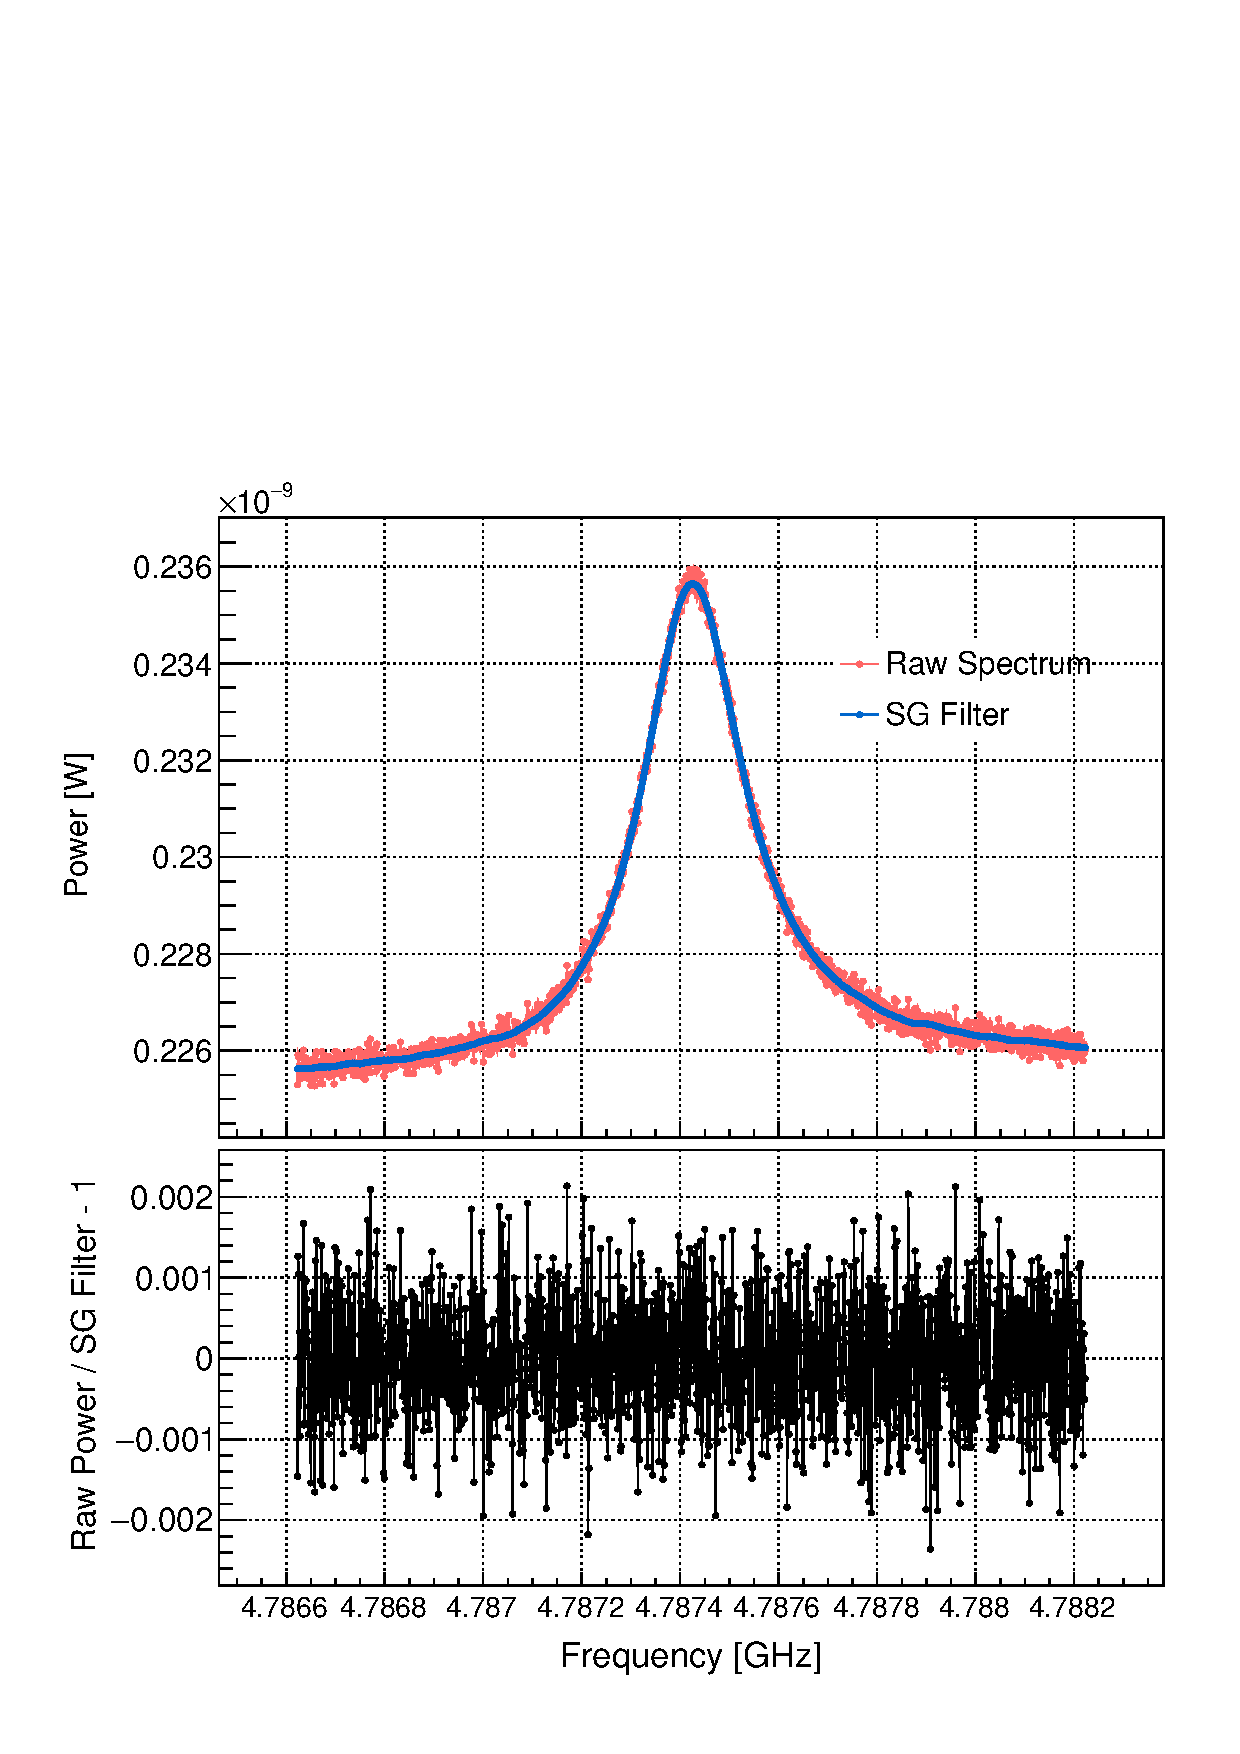
\includegraphics[width=6.5cm]{figures/RawPower_SGPower_Ratio_vs_Freq_Step_0100.pdf}
  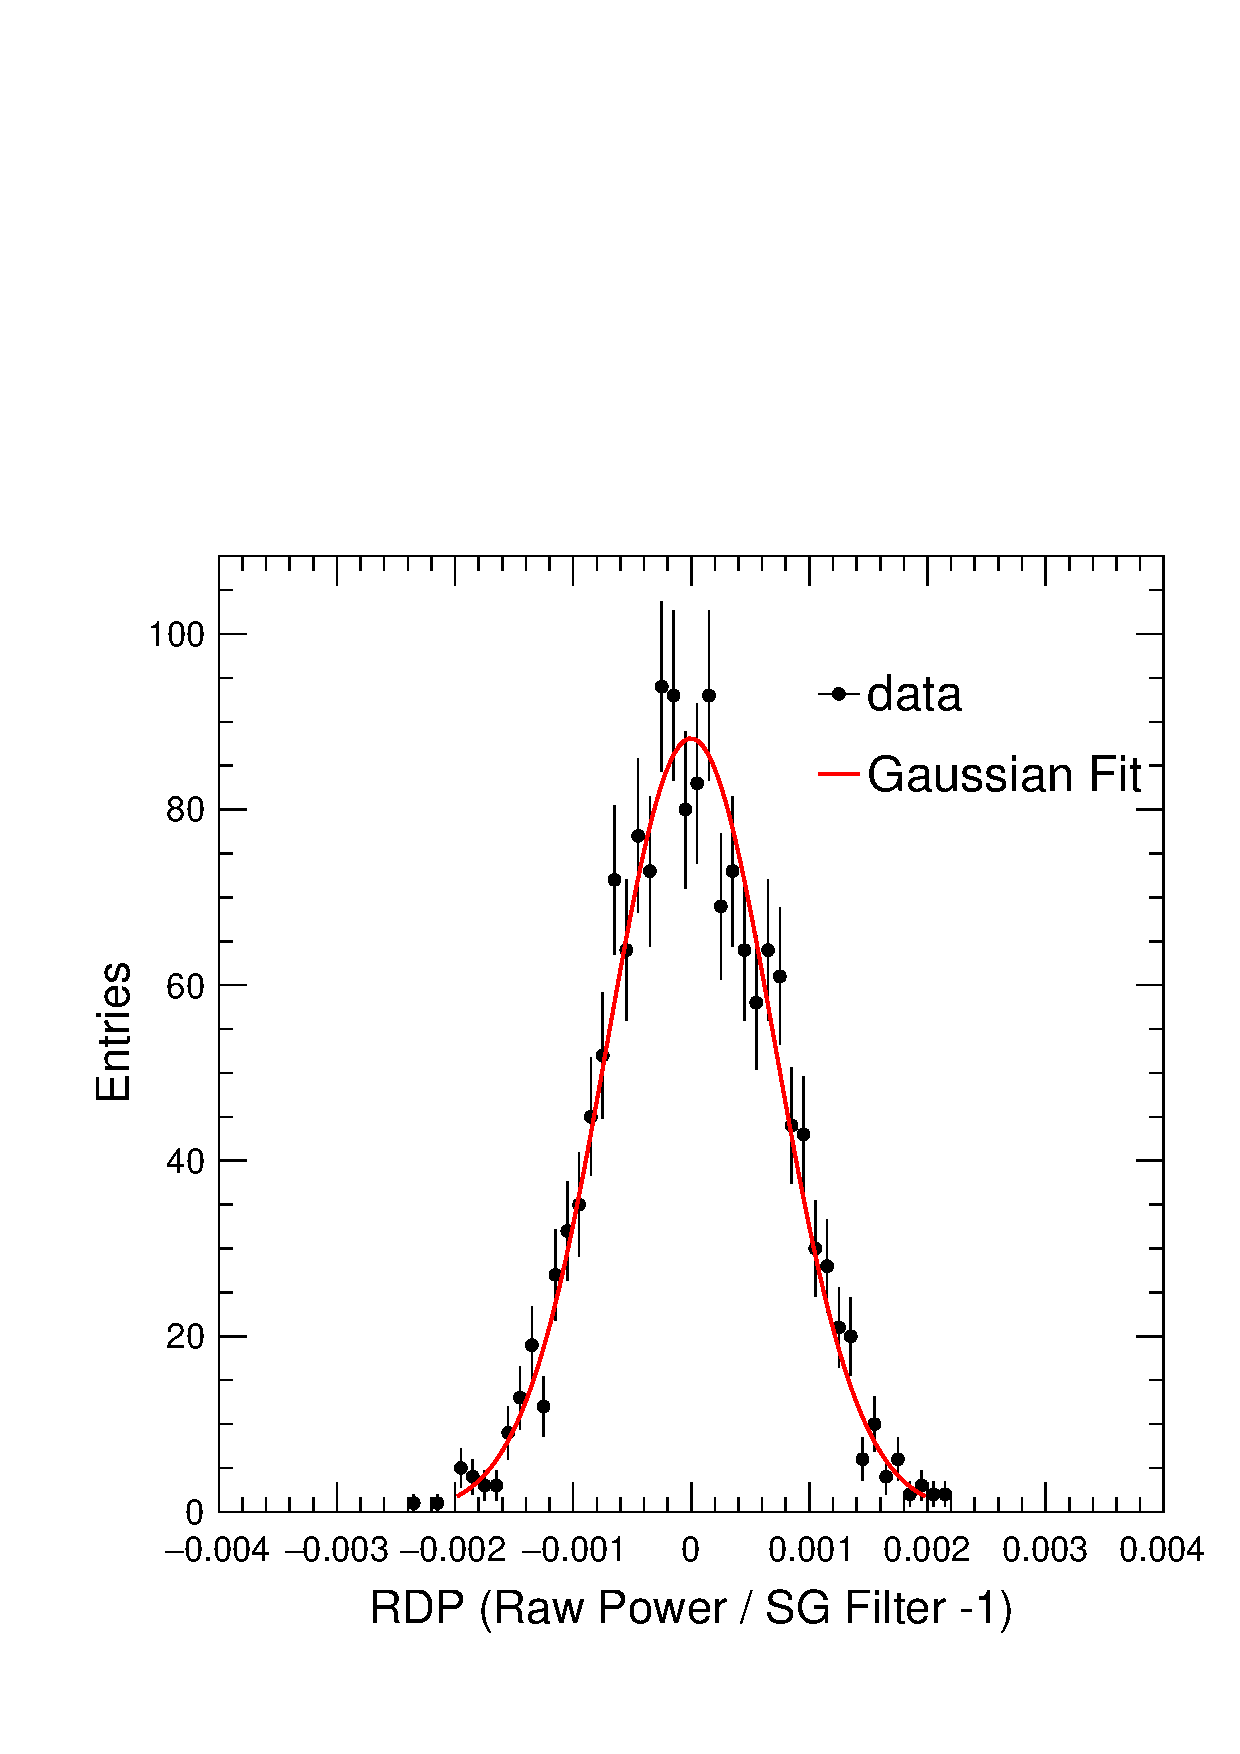
\includegraphics[width=6.5cm]{figures/Histogram_RawPower_SGPower_Ratio_Step_0100.pdf}
  \caption{Upper left panel: The raw averaged power spectrum (red points) and the 
output of the SG filter (blue curve) of one scan. Lower left panel: The normalized 
spectrum,  derived by taking the ratio of the raw spectrum to the SG filter 
and subtracting unity from the ratio.
Right plot: Histogram of the normalized spectrum (lower panel in left plot) with a Gaussian 
fit; there are 1600 entries in total (from the 1600 frequency bins). 
The fitted mean and standard deviation are shown to be consistent with the prediction 
when the axion signal is not present.}
  \label{fig:raw_sg_power}
\end{figure*}


\subsection{Combine the spectra with the weighting algorithm} 
\label{sec:weighting_algorithm}
During the data taking, the resonant frequency of the cavity was  
adjusted by the tuning bar to scan a large range of frequencies.  
Therefore, the spectra of all the scans need to be combined to create one 
big spectrum. 
The purpose of the weighting algorithm is to add the spectra from different 
resonant-frequency scans,
 particularly for the frequency bins that appear in multiple spectra. 
Note that the uncertainty of the averaged power at the overlapped region is 
reduced due to the combination.  
The weight is defined below: 
\begin{equation}
    \label{eq:weight}
    {w_{ijn}} = \frac{\Gamma_{ijn}}{(\sigma_{ij}^\text{res})^{2}}.
\end{equation}
Here, the symbol $\Gamma_{ijn}=1$ if the $j^\text{th}$ frequency bin in the 
$i^\text{th}$ rescaled spectrum correspond to the same frequency in 
the $n^\text{th}$ bin of the combined spectrum; otherwise, $\Gamma_{ijn}=0$.

The RDP $\delta^\text{com}_{n}$ and the standard deviation 
$\sigma^\text{com}_{n}$ of the $n^\text{th}$ bin in the combined spectrum are 
calculated using Eq.~\eqref{eq:comb_power} and Eq.~\eqref{eq:comb_sigma}, 
respectively. The notation SNR$^\text{com}_{n}$ is the ratio of 
$\delta^\text{com}_{n}$ to 
$\sigma^\text{com}_{n}$ as given in Eq.~\eqref{eq:comb_snr}. 
Figure~\ref{fig:SNR_comb} shows the SNR of the combined spectrum. 

\begin{equation}
    \label{eq:comb_power}
    \delta_{n}^\text{com} = \frac{\sum\limits_{i}\sum\limits_{j}\left(\delta_{ij}^\text{res} \cdot {w_{ijn}}\right)}{\sum\limits_{i}\sum\limits_{j} {w_{ijn}}},
\end{equation}

\begin{equation}
    \label{eq:comb_sigma}
    \sigma_{n}^\text{com} = \frac{ \sqrt{\sum\limits_{i}\sum\limits_{j}(\sigma_{ij}^\text{res} \cdot {w_{ijn}})^2}}{\sum\limits_{i}\sum\limits_{j} {w_{ijn}}},
\end{equation}
\begin{equation}
    \label{eq:comb_snr}
    \text{SNR}_{n}^\text{com} = \frac{\delta^\text{com}_{n}}{\sigma^\text{com}_{n}}= \frac{\sum\limits_{i}\sum\limits_{j}\left(\delta_{ij}^\text{res} \cdot {w_{ijn}}\right)}{ \sqrt{\sum\limits_{i}\sum\limits_{j}(\sigma_{ij}^\text{res} \cdot {w_{ijn}})^2}}.
\end{equation} 
The summations over $i$ run from 1 to 837 (steps) while the summations 
over $j$ run from 1 to 1600 (bins).  
For each bin $n$ in the combined spectrum, there are $m_n$ non-vanishing 
contributions to the sums above. In general, the value of $m_n$ is 14--16.


\begin{figure}[hbt!]
    \centering
    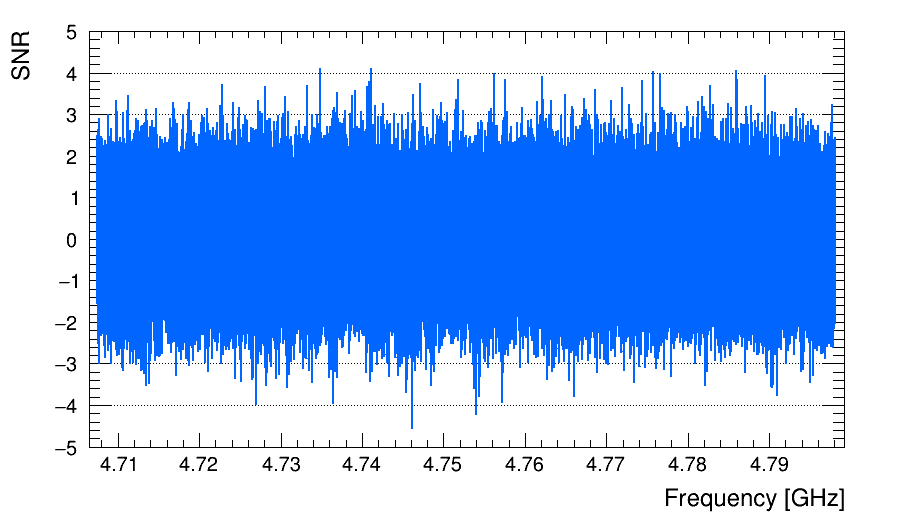
\includegraphics[width=8.6cm]{figures/SNR_CombSpectrum_AxionRun_AllSteps_Rescan_SG4_W201_LqWeight.png}
    \caption{The signal-to-noise ratio (SNR) calculated using 
Eq.\eqref{eq:comb_snr} of the combined spectrum. }
    \label{fig:SNR_comb}
\end{figure}

\subsection{Merge bins}
\label{sec:merge}

The expected axion bandwidth is about 5~kHz at the frequency of 
$\approx5$~GHz. 
In this paper, the interested frequency range is \flo -- \fhi~GHz and the bin 
width is 1~kHz. Therefore, in order to maximize the SNR, a running window of 
five consecutive bins in the combined spectrum is applied and the five bins 
within each window are merged to construct a final spectrum.  
The purpose of using a running window is to avoid the signal power broken 
into different neighboring bins of the merged spectrum. 
The number of bins for merging is studied by injecting 
simulated axion signals on top of the CD102 data and optimized based 
on the SNR. 

Due to the nonuniform distribution of the axion signal 
[Eq.~\eqref{eq:simplesignal}],
the contributing bins need to be rescaled to have the same RDP, of which the 
standard deviation is used to define the maximum likelihood (ML)
weight for merging. The rescaling is performed by dividing the values of 
$\delta^\text{com}_{g+k-1}$ and $\sigma^\text{com}_{g+k-1}$ in the combined 
spectrum with an integral of the signal line shape $L_{k}$:

\begin{equation}
  \label{eq:Lq_integral}
  L_{k} = \int_{f_a +\delta f_m + (k-1)\Delta f_\text{bin}}^{f_a +\delta f_m + k\Delta f_\text{bin}} \mathcal{F}(f,f_a) \,df,
\end{equation}
where the variable $g$ is the index for the frequency bins in 
the final merged spectrum and 
$k$ is the index within the group of bins for 
merging. The index $g$ runs from 1 to $N-M+1$, where 
the number $N$ is the total number of bins in 
the combined spectrum and $M=5$ is the number of 
merged bin in this analysis. 
The frequency $f_a=\left.\ma c^2\middle/h\right.$ is the axion
frequency, and $\delta f_m$ is the misalignment between $f_a$ and the lower
boundary of the $g^\text{th}$ bin in the merged spectrum.
The function $\mathcal{F}(f,f_a)$ has been defined in 
Eq.~\eqref{eq:simplesignal}.
In order to get a misalignment-independent line shape, instead of using an
$L_{k}$ that depends on the frequency $f_a$ and  $\delta f_m$, the average 
($\bar{L}_{k}$) of $L_{k}$ over the ranges of $f_a$ and $\delta f_m$ is 
used. 
Note that the relative variation of $f_a$ is at most 
90~MHz/5~GHz$\approx2\%$ and the line shape of $\mathcal{F}(f,f_a)$ 
can be considered constant for the full range of the operational 
frequency. Therefore, 
the value of $L_{k}$ has only weak dependence on $f_a$. 
In the analysis presented here, 
$\bar{L}_{k} = 0.23, 0.33, 0.21, 0.11, 0.06$ for $k = 1, ... 5$, respectively.
The effect of the misalignment on the \gagg\ limits is quoted as a part of 
the systematic uncertainty using the same method as described in the HAYSTAC 
paper~\cite{HAYSTACII}, see Sec.~\ref{sec:sys}.

The rescaled RDP $\delta^\text{rs}_{g+k-1}$ and
standard deviation $\sigma^\text{rs}_{g+k-1}$ are calculated:
\begin{equation}
  \label{eq:rescaled_delta_sigma_com}
  \begin{split}
  \delta^\text{rs}_{g+k-1} = \frac{\delta^\text{com}_{g+k-1}}{\bar{L}_{k}},\\
  \sigma^\text{rs}_{g+k-1} = \frac{\sigma^\text{com}_{g+k-1}}{\bar{L}_{k}}.
  \end{split}
\end{equation}
After this rescaling 
procedure, a KSVZ axion signal is expected to have an RDP equal to unity for 
each of the five bins. 
The ML weight is defined as: 
\begin{equation}
    \label{eq:merge_weight}
    w_{gk} = \frac{1}{(\sigma_{g+k-1}^\text{rs})^{2}} = \frac{\bar{L}_{k}^{2}}{(\sigma_{g+k-1}^\text{com})^{2}}.
\end{equation}

The RDP, the standard deviation, and the SNR of the merged spectrum are:

\begin{equation}
    \delta_{g}^\text{merged} = \frac{ \sum\limits_{k = 1}^{M}\left(\delta_{g+k-1}^\text{rs} \cdot {w_{gk}}\right)}{\sum\limits_{k = 1}^{M} {w_{gk}}} = \frac{\sum\limits_{k = 1}^{M}\frac{\delta_{g+k-1}^\text{com}}{\bar{L}_{k}} \cdot \left(\frac{\bar{L}_{k}}{\sigma_{g+k-1}^\text{com}}\right)^2} {\sum\limits_{k = 1}^{M}\left(\frac{\bar{L}_{k}}{\sigma_{g+k-1}^\text{com}}\right)^2},
    \label{eq:merged_power}
\end{equation}

\begin{eqnarray}
  \sigma_{g}^\text{merged} & =  & \frac{ \sqrt{\sum\limits_{k = 1}^{M} \left(\sigma_{g+k-1}^\text{rs} \cdot {w_{gk}}\right)^2}}{\sum\limits_{k = 1}^{M} {w_{gk}}} = \frac{\sqrt{\sum\limits_{k = 1}^{M} \left(\frac{\bar{L}_{k}}{\sigma_{g+k-1}^\text{com}}\right)^2}}{\sum\limits_{k = 1}^{M} \left(\frac{\bar{L}_{k}}{\sigma_{g+k-1}^\text{com}}\right)^2}  \nonumber \\
    & = & \frac{1}{\sqrt{\sum\limits_{k = 1}^{M} \left(\frac{\bar{L}_{k}}{\sigma_{g+k-1}^\text{com}}\right)^2}}
    \label{eq:merged_sigma}
\end{eqnarray}

\begin{equation}
    \label{eq:merged_snr}
    \text{SNR}_{g}^\text{merged} = \frac{\delta^\text{merged}_{g}}{\sigma^\text{merged}_{g}} = \frac{\sum\limits_{k = 1}^{M}\frac{\delta_{g+k-1}^\text{com}}{\bar{L}_{k}} \cdot \left(\frac{\bar{L}_{k}}{\sigma_{g+k-1}^\text{com}}\right)^2}{\sqrt{\sum\limits_{k = 1}^{M} \left(\frac{\bar{L}_{k}}{\sigma_{g+k-1}^\text{com}}\right)^2}}
\end{equation}


\subsection{Rescan and set limits on \gagg} 
Before the collection of the CD102 data, a 5$\sigma$ SNR target was chosen, 
which corresponds to a candidate threshold of 3.355$\sigma$ at 95\% C.L..
 After the merging as described in Sec.~\ref{sec:merge}, if there were 
any potential signal with an SNR larger than 
3.355, a rescan would be proceeded to check if it were a real signal 
or a statistical fluctuation. 
The procedure of the CD102 data taking was to perform a rescan after 
covering every 10~MHz; the rescan was done by adjusting the tuning rod of the 
cavity so to match the resonant frequency to the frequency of the candidate. 
In total, 22 candidates with an SNR greater than 3.355 were found. 
Among them, 20 candidates were from the fluctuations because they were gone 
after a few rescans. The remaining two candidates, 
in the frequency ranges of 4.71017 -- 4.71019~GHz and 4.74730 -- 4.74738~GHz, 
are excluded from consideration of axion signal candidates due to the 
following reasons. 
The signal in the second frequency range 
was detected via a portable antenna outside the DR and found 
to come from the instrument control computer in the laboratory, while the 
signal in the first frequency range 
was not detected outside the DR but 
still present after turning off the external magnetic field. 
No limits are placed for the two frequency ranges above.  
More details can be found in the 
TASEH instrumentation paper~\cite{TASEHInstrumentation}. 
Figure~\ref{fig:SNR_merged} shows the SNR of the merged spectrum after 
including data from both the original scans and the rescans. 

Since no candidates were found after the rescan, an upper limit on 
the signal power $P_s$ is derived by setting $P_s$ equal to 
$5\sigma_{g}^\text{merged}\times P_{g}^\text{KSVZ}$, where 
$\sigma_{g}^\text{merged}$ is the standard deviation 
and $P_{g}^\text{KSVZ}$ is the expected signal power for the KSVZ axion 
for a certain frequency bin $g$ in the merged spectrum. 
Then, the 95\% C.L. limits on the dimensionless parameter 
\ggamma\ and the axion-two-photon coupling \gagg\ could be derived 
according to Eq.~\eqref{eq:ps} and Eq.~\eqref{eq:grelation}. 
See Sec.~\ref{sec:results} for the final limits including the systematic 
uncertainties.


\begin{figure}[hbt!]
    \centering
    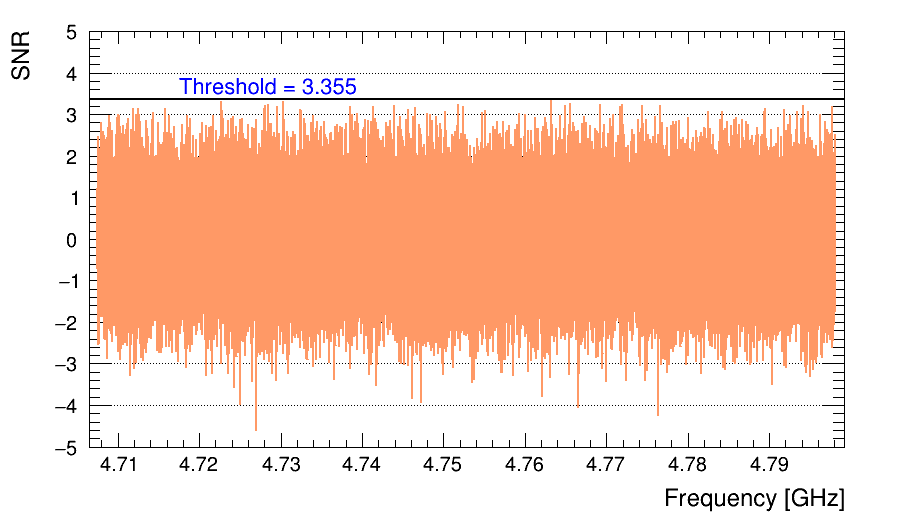
\includegraphics[width=8.6cm]{figures/SNR_GrandSpectrum_AxionRun_AllSteps_Rescan_Merged_5bin_SG4_W201_LqWeight.png}
    \caption{The signal-to-noise ratio (SNR) calculated using Eq.~\eqref{eq:merged_snr} for the merged spectrum including data from both the original 
scans and the rescans. No candidate exceeds the threshold of 
$3.355\sigma$ (solid-black horizontal line). }
    \label{fig:SNR_merged}
\end{figure}
